% GNUPLOT: LaTeX picture with Postscript
\begingroup
  \makeatletter
  \providecommand\color[2][]{%
    \GenericError{(gnuplot) \space\space\space\@spaces}{%
      Package color not loaded in conjunction with
      terminal option `colourtext'%
    }{See the gnuplot documentation for explanation.%
    }{Either use 'blacktext' in gnuplot or load the package
      color.sty in LaTeX.}%
    \renewcommand\color[2][]{}%
  }%
  \providecommand\includegraphics[2][]{%
    \GenericError{(gnuplot) \space\space\space\@spaces}{%
      Package graphicx or graphics not loaded%
    }{See the gnuplot documentation for explanation.%
    }{The gnuplot epslatex terminal needs graphicx.sty or graphics.sty.}%
    \renewcommand\includegraphics[2][]{}%
  }%
  \providecommand\rotatebox[2]{#2}%
  \@ifundefined{ifGPcolor}{%
    \newif\ifGPcolor
    \GPcolortrue
  }{}%
  \@ifundefined{ifGPblacktext}{%
    \newif\ifGPblacktext
    \GPblacktexttrue
  }{}%
  % define a \g@addto@macro without @ in the name:
  \let\gplgaddtomacro\g@addto@macro
  % define empty templates for all commands taking text:
  \gdef\gplbacktext{}%
  \gdef\gplfronttext{}%
  \makeatother
  \ifGPblacktext
    % no textcolor at all
    \def\colorrgb#1{}%
    \def\colorgray#1{}%
  \else
    % gray or color?
    \ifGPcolor
      \def\colorrgb#1{\color[rgb]{#1}}%
      \def\colorgray#1{\color[gray]{#1}}%
      \expandafter\def\csname LTw\endcsname{\color{white}}%
      \expandafter\def\csname LTb\endcsname{\color{black}}%
      \expandafter\def\csname LTa\endcsname{\color{black}}%
      \expandafter\def\csname LT0\endcsname{\color[rgb]{1,0,0}}%
      \expandafter\def\csname LT1\endcsname{\color[rgb]{0,1,0}}%
      \expandafter\def\csname LT2\endcsname{\color[rgb]{0,0,1}}%
      \expandafter\def\csname LT3\endcsname{\color[rgb]{1,0,1}}%
      \expandafter\def\csname LT4\endcsname{\color[rgb]{0,1,1}}%
      \expandafter\def\csname LT5\endcsname{\color[rgb]{1,1,0}}%
      \expandafter\def\csname LT6\endcsname{\color[rgb]{0,0,0}}%
      \expandafter\def\csname LT7\endcsname{\color[rgb]{1,0.3,0}}%
      \expandafter\def\csname LT8\endcsname{\color[rgb]{0.5,0.5,0.5}}%
    \else
      % gray
      \def\colorrgb#1{\color{black}}%
      \def\colorgray#1{\color[gray]{#1}}%
      \expandafter\def\csname LTw\endcsname{\color{white}}%
      \expandafter\def\csname LTb\endcsname{\color{black}}%
      \expandafter\def\csname LTa\endcsname{\color{black}}%
      \expandafter\def\csname LT0\endcsname{\color{black}}%
      \expandafter\def\csname LT1\endcsname{\color{black}}%
      \expandafter\def\csname LT2\endcsname{\color{black}}%
      \expandafter\def\csname LT3\endcsname{\color{black}}%
      \expandafter\def\csname LT4\endcsname{\color{black}}%
      \expandafter\def\csname LT5\endcsname{\color{black}}%
      \expandafter\def\csname LT6\endcsname{\color{black}}%
      \expandafter\def\csname LT7\endcsname{\color{black}}%
      \expandafter\def\csname LT8\endcsname{\color{black}}%
    \fi
  \fi
    \setlength{\unitlength}{0.0500bp}%
    \ifx\gptboxheight\undefined%
      \newlength{\gptboxheight}%
      \newlength{\gptboxwidth}%
      \newsavebox{\gptboxtext}%
    \fi%
    \setlength{\fboxrule}{0.5pt}%
    \setlength{\fboxsep}{1pt}%
    \definecolor{tbcol}{rgb}{1,1,1}%
\begin{picture}(6180.00,4460.00)%
    \gplgaddtomacro\gplbacktext{%
      \csname LTb\endcsname%%
      \put(1065,841){\makebox(0,0)[r]{\strut{}$-150$}}%
      \csname LTb\endcsname%%
      \put(1065,1307){\makebox(0,0)[r]{\strut{}$-100$}}%
      \csname LTb\endcsname%%
      \put(1065,1772){\makebox(0,0)[r]{\strut{}$-50$}}%
      \csname LTb\endcsname%%
      \put(1065,2237){\makebox(0,0)[r]{\strut{}$0$}}%
      \csname LTb\endcsname%%
      \put(1065,2702){\makebox(0,0)[r]{\strut{}$50$}}%
      \csname LTb\endcsname%%
      \put(1065,3167){\makebox(0,0)[r]{\strut{}$100$}}%
      \csname LTb\endcsname%%
      \put(1065,3633){\makebox(0,0)[r]{\strut{}$150$}}%
      \csname LTb\endcsname%%
      \put(1442,386){\makebox(0,0){\strut{}$-150$}}%
      \csname LTb\endcsname%%
      \put(1907,386){\makebox(0,0){\strut{}$-100$}}%
      \csname LTb\endcsname%%
      \put(2372,386){\makebox(0,0){\strut{}$-50$}}%
      \csname LTb\endcsname%%
      \put(2838,386){\makebox(0,0){\strut{}$0$}}%
      \csname LTb\endcsname%%
      \put(3303,386){\makebox(0,0){\strut{}$50$}}%
      \csname LTb\endcsname%%
      \put(3768,386){\makebox(0,0){\strut{}$100$}}%
      \csname LTb\endcsname%%
      \put(4233,386){\makebox(0,0){\strut{}$150$}}%
    }%
    \gplgaddtomacro\gplfronttext{%
      \csname LTb\endcsname%%
      \put(2838,123){\makebox(0,0){\strut{}$\Phi$}}%
      \csname LTb\endcsname%%
      \put(4861,562){\makebox(0,0)[l]{\strut{}$0$}}%
      \csname LTb\endcsname%%
      \put(4861,1041){\makebox(0,0)[l]{\strut{}$0.5$}}%
      \csname LTb\endcsname%%
      \put(4861,1519){\makebox(0,0)[l]{\strut{}$1$}}%
      \csname LTb\endcsname%%
      \put(4861,1998){\makebox(0,0)[l]{\strut{}$1.5$}}%
      \csname LTb\endcsname%%
      \put(4861,2476){\makebox(0,0)[l]{\strut{}$2$}}%
      \csname LTb\endcsname%%
      \put(4861,2955){\makebox(0,0)[l]{\strut{}$2.5$}}%
      \csname LTb\endcsname%%
      \put(4861,3433){\makebox(0,0)[l]{\strut{}$3$}}%
      \csname LTb\endcsname%%
      \put(4861,3912){\makebox(0,0)[l]{\strut{}$3.5$}}%
      \csname LTb\endcsname%%
      \put(1348,3308){\rotatebox{18.00}{\makebox(0,0){\small 2.70}}}%
      \csname LTb\endcsname%%
      \put(1466,2373){\rotatebox{-131.00}{\makebox(0,0){\small 2.70}}}%
      \csname LTb\endcsname%%
      \put(4361,3027){\rotatebox{-120.00}{\makebox(0,0){\small 2.70}}}%
      \csname LTb\endcsname%%
      \put(3990,1831){\rotatebox{-124.00}{\makebox(0,0){\small 2.70}}}%
      \csname LTb\endcsname%%
      \put(2139,3784){\rotatebox{1.00}{\makebox(0,0){\small 2.21}}}%
      \csname LTb\endcsname%%
      \put(2593,2833){\rotatebox{-29.00}{\makebox(0,0){\small 2.21}}}%
      \csname LTb\endcsname%%
      \put(3351,1938){\rotatebox{-63.00}{\makebox(0,0){\small 2.21}}}%
      \csname LTb\endcsname%%
      \put(4089,2346){\rotatebox{62.00}{\makebox(0,0){\small 2.21}}}%
      \csname LTb\endcsname%%
      \put(1550,2043){\rotatebox{73.00}{\makebox(0,0){\small 2.21}}}%
      \csname LTb\endcsname%%
      \put(2274,2647){\rotatebox{-55.00}{\makebox(0,0){\small 2.21}}}%
      \csname LTb\endcsname%%
      \put(2981,1705){\rotatebox{-29.00}{\makebox(0,0){\small 2.21}}}%
      \csname LTb\endcsname%%
      \put(3435,699){\rotatebox{-16.00}{\makebox(0,0){\small 2.21}}}%
      \csname LTb\endcsname%%
      \put(1695,1656){\rotatebox{83.00}{\makebox(0,0){\small 1.72}}}%
      \csname LTb\endcsname%%
      \put(2459,2104){\rotatebox{-61.00}{\makebox(0,0){\small 1.72}}}%
      \csname LTb\endcsname%%
      \put(2895,1017){\rotatebox{-103.00}{\makebox(0,0){\small 1.72}}}%
      \csname LTb\endcsname%%
      \put(2878,3642){\rotatebox{-129.00}{\makebox(0,0){\small 1.72}}}%
      \csname LTb\endcsname%%
      \put(3142,2565){\rotatebox{-54.00}{\makebox(0,0){\small 1.72}}}%
      \csname LTb\endcsname%%
      \put(3952,2582){\rotatebox{74.00}{\makebox(0,0){\small 1.72}}}%
      \csname LTb\endcsname%%
      \put(1264,904){\rotatebox{32.00}{\makebox(0,0){\small 1.24}}}%
      \csname LTb\endcsname%%
      \put(1971,1846){\rotatebox{41.00}{\makebox(0,0){\small 1.24}}}%
      \csname LTb\endcsname%%
      \put(2631,1050){\rotatebox{-112.00}{\makebox(0,0){\small 1.24}}}%
      \csname LTb\endcsname%%
      \put(3958,3828){\rotatebox{-142.00}{\makebox(0,0){\small 1.24}}}%
      \csname LTb\endcsname%%
      \put(3026,3154){\rotatebox{-73.00}{\makebox(0,0){\small 1.24}}}%
      \csname LTb\endcsname%%
      \put(3805,2822){\rotatebox{73.00}{\makebox(0,0){\small 1.24}}}%
      \csname LTb\endcsname%%
      \put(1701,1109){\rotatebox{49.00}{\makebox(0,0){\small 0.75}}}%
      \csname LTb\endcsname%%
      \put(2344,1084){\rotatebox{-146.00}{\makebox(0,0){\small 0.75}}}%
      \csname LTb\endcsname%%
      \put(3723,3525){\rotatebox{-158.00}{\makebox(0,0){\small 0.75}}}%
      \csname LTb\endcsname%%
      \put(3738,3076){\rotatebox{54.00}{\makebox(0,0){\small 0.75}}}%
      \csname LTb\endcsname%%
      \put(2838,4176){\makebox(0,0){\strut{}Dipole field (Debye)}}%
    }%
    \gplbacktext
    \put(0,0){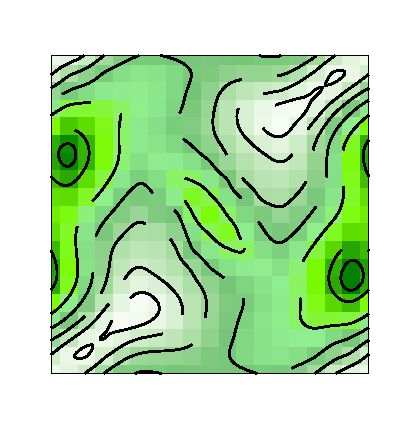
\includegraphics[width={309.00bp},height={223.00bp}]{Q0_d}}%
    \gplfronttext
  \end{picture}%
\endgroup
